\subsection{Описание используемых паттернов проектирования}
\label{sec:modeling:patterns}

Шаблон проектирования или паттерн в разработке программного обеспечения — повторяемая архитектурная конструкция, представляющая собой решение проблемы проектирования в рамках некоторого часто возникающего контекста.

Обычно шаблон не является законченным образцом, который может быть прямо преобразован в код; это лишь пример решения задачи, который можно использовать в различных ситуациях. Объектно-ориентированные шаблоны показывают отношения и взаимодействия между классами или объектами, без определения того, какие конечные классы или объекты приложения будут использоваться.

<<Низкоуровневые>> шаблоны, учитывающие специфику конкретного языка программирования, называются идиомами. Это хорошие решения проектирования, характерные для конкретного языка или программной платформы, и потому не универсальные.

На наивысшем уровне существуют архитектурные шаблоны, они охватывают собой архитектуру всей программной системы. Алгоритмы по своей сути также являются шаблонами, но не проектирования, а вычисления, так как решают вычислительные задачи. В сравнении с полностью самостоятельным проектированием, шаблоны обладают рядом преимуществ. Основная польза от использования шаблонов состоит в снижении сложности разработки за счёт готовых абстракций для решения целого класса проблем. 

Шаблон даёт решению своё имя, что облегчает коммуникацию между разработчиками, позволяя ссылаться на известные шаблоны. Таким образом, за счёт шаблонов производится унификация деталей решений: модулей, элементов проекта, — снижается количество ошибок. Применение шаблонов концептуально сродни использованию готовых библиотек кода.

Правильно сформулированный шаблон проектирования позволяет, отыскав удачное решение, пользоваться им снова и снова. Набор шаблонов помогает разработчику выбрать возможный, наиболее подходящий вариант проектирования. 

Хотя легкое изменение кода под известный шаблон может упростить понимание кода, по мнению Стива Макконнелла, с применением шаблонов могут быть связаны две сложности. Во-первых, слепое следование некоторому выбранному шаблону может привести к усложнению программы. Во-вторых, у разработчика может возникнуть желание попробовать некоторый шаблон в деле без особых оснований. 

\subsubsection{}Одиночка
\

В данном программном средстве используется паттерн <<Одиночка>>.
Одиночка (англ. Singleton) — порождающий шаблон проектирования, гарантирующий, что в однопроцессном приложении будет единственный экземпляр некоторого класса, и предоставляющий глобальную точку доступа к этому экземпляру. У класса есть только один экземпляр, и он предоставляет к нему глобальную точку доступа~\cite{design_patterns}. Краткое описание паттерна представлено на рисунке~\ref{sec:modeling:singleton}.

\begin{figure}[ht]
\centering
    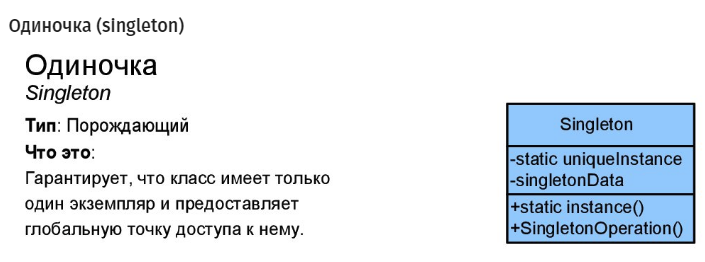
\includegraphics[scale=0.6]{design_singleton_pattern.png}
    \caption{Паттерн проектирования <<Одиночка>>}
    \label{sec:modeling:singleton}
\end{figure}

Существенно то, что можно пользоваться именно экземпляром класса, так как при этом во многих случаях становится доступной более широкая функциональность. Например, к описанным компонентам класса можно обращаться через интерфейс, если такая возможность поддерживается языком.

Глобальный <<одинокий>> объект — именно объект, а не набор процедур, не привязанных ни к какому объекту — бывает нужен:

\begin{itemize}
    \item если используется существующая объектно-ориентированная библиотека;
    \item если есть шансы, что один объект когда-нибудь превратится в несколько;
    \item если интерфейс объекта (например, игрового мира) слишком сложен и не стоит засорять основное пространство имён большим количеством функций;
    \item если, в зависимости от каких-нибудь условий и настроек, создаётся один из нескольких объектов. Например, в зависимости от того, ведётся лог или нет, создаётся или настоящий объект, пишущий в файл, или <<заглушка>>, ничего не делающая.
\end{itemize}

Минусы:
\begin{itemize}
    \item если объект нужен уже при инициализации, он может быть затребован раньше, чем будет создан;
    \item бывает, что объект нужен не всегда. В таком случае его создание можно пропустить.
\end{itemize}

\subsubsection{}Фабрика
\

Factory -- это паттерн создания объектов (creational pattern). Данный шаблон проектирования предоставляет интерфейс для создания экземпляров некоторого класса~\cite{design_patterns}. В момент создания наследники могут определить, какой класс инстанциировать. Краткое описание паттерна представлено на рисунке~\ref{sec:modeling:factory}.

\begin{figure}[ht]
\centering
    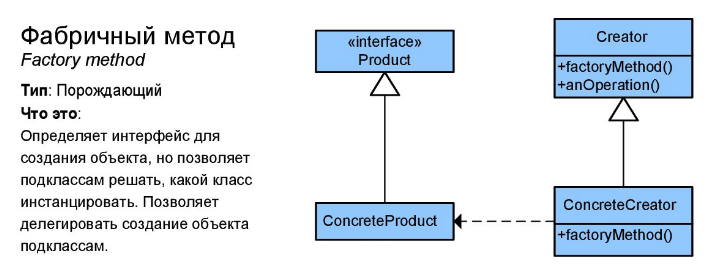
\includegraphics[scale=0.6]{design_factory_pattern.png}
    \caption{Паттерн проектирования <<Фабрика>>}
    \label{sec:modeling:factory}
\end{figure}

Иными словами, Фабрика делегирует создание объектов наследникам родительского класса. Это позволяет использовать в коде программы не специфические классы, а манипулировать абстрактными объектами на более высоком уровне.